\section{GNOME}
\label{sec:gnome}

\par \textbf{GNOME} is an acronym that means: \textit{GNU Object Model Environment}. Was created in 1997 through the visible momentum of \textit{\href{http://tirania.org/blog/}{Miguel de Icaza}} to provide graphical desktop environments completely FLOSS Linux version build using components and focused on interoperability. Counteract the existing KDE fed on QT (at that time \textbf{was proprietary software, not now}). After some analysis they start developing GNOME using GTK (\textit{\href{http://www.gimp.org/}{Gimp Toolkit}, yes Gimp GNU Image Manipulation Program}:)).

\par \textit{GNOME Foundation} was founded on 15 August 2000 by Compaq, Eazel, Helix Code, IBM, Red Hat and Sun Microsystems. Manages GNOME development and represents GNOME worldwide.

\subsection{Technologies}

\par GNOME is developed using C language and Object Oriented GTK+ library. Each project/module is governed by these basic development tools:

\begin{itemize}
	\item \textit{Maintainer} - benevolent dictator for life for each module. GNOME has a distributed development management divided in modules.
	\item \textit{Mailing list} - Encourage users to develop discussions in mailing list instead of IRC because it is easier to manage the history of the decisions made. \href{https://mail.gnome.org/mailman/listinfo}{Mailing Lists}.
	\item \textit{Bug Tracking System} - \href{https://bugzilla.gnome.org/}{GNOME Bugzilla} manages Project development, Bugs and discussions.
	\item \textit{Documentation} - Wiki is a very useful tool in project development because brings information from the project and its easier to use as a collaborative document development for technical and non-technical users. GNOME Wiki is published in \url{https://live.gnome.org/}.
	\item \textit{Repository} - Distributed repository git in \url{https://git.gnome.org/browse/} and a user guide that explains the use of the repository in live \href{https://live.gnome.org/Git}{Wiki}.
	\item \textit{Synchronous communication} - IRC channel to retrieve information and ask questions related to GNOME. You can find more information in \href{https://live.gnome.org/GnomeIrcChannels}{Wiki} IRC section.
	\item \textit{Quality and Assurance} - Users, the users are the best QA team for Gnome.
\end{itemize} There is a manual for developers specifically dedicated to them, \href{https://developer.gnome.org/}{GNOME Developer Center}. In showing a series of tutorials, documentation and GNOME structure to facilitate the use and implementation of the platform.

\begin{figure}[H]
    \centering
    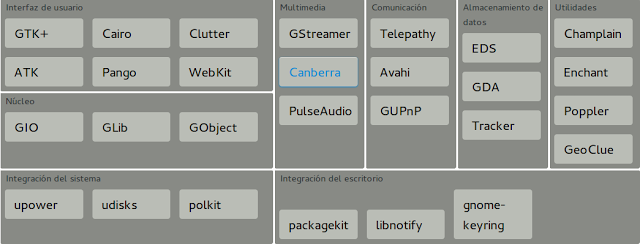
\includegraphics[width=0.7\textwidth]{gnome-system-modules}
    \caption{Gnome platform overview}
    \label{platform}
\end{figure}

\subsection{How to Contribute}

\par GNOME Community has a low barrier entrance guided by Meritocracy. Community guides are available to everyone in \href{https://live.gnome.org/GnomeLove}{GnomeLove}. Here we are going to describe internal process of a contribution and how a contributor reaches the goal of becoming a commiter througth different organization ROLES:

\begin{itemize}
	\item Reasonable number of patches in a module.
	\item Ask for commit rights to Accounts Team
	\item Accounts Team contact module maintainer or translator coordinator to check for approval.
	\item A committer can commit to git repository but her contributions have to be reviewed and approved by maintainer of the module
	\item \textbf{Important}: committers have write access to all git repositories hosted in git.gnome.org. You can contribute to all modules. If you find an error you could fix and commit the patch.
\end{itemize}

\par \textit{Maintainers} are responsible for the module. They have to \textit{review patches} and \textit{assume results}, their role is important inside the community have high responsability. Communications and module releases management are managed by maintainers. Could be various maintainers for one module.

\par Instead of development committers, translators committers in translation modules also are maintainers for themselves because \textit{a translation can't be reviewed} because \textit{it would duplicate the work}. So you have full confidence in the translation module.

% section gnome (end)